%!TEX root = ../main.tex
%%%%%%%%%%%%%%%%%%%%%%%%%%%%%%%%%%
% Links:
%
% Difficulty:
% Companies: 
%%%%%%%%%%%%%%%%%%%%%%%%%%%%%%%%%%


%\begin{figure}
%	\centering
%	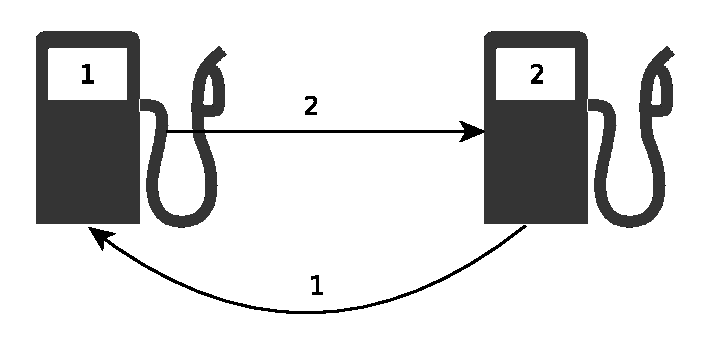
\includegraphics[width=\textwidth]{sources/gas_station/images/example1}
%	\caption[Sample short cpation]{Sample Caption}.
%	\label{fig:gas_station:example1}
%\end{figure}

\chapter{Gas Station \faGasPump}
\label{ch:gas_station}
\section*{Introduction}
Imagine there we drive along a circular route with a number of gas stations along it. Our goal is to drive across the entire route but before departure we would like to make sure we are not going to get stranded because we run out of gas.

Our car starts with an empty tank and can make 1km per 1l of gas and each gas station has a maximum amount of gas it can deliver. 
The problem with this setting is that we can end up in a situation where after 
having refueled we still do not have enough gas to reach the next gas station. 

In the problem discussed in this chapter we will discuss how to make sure  we always start the journey from a place along the route from where it is not possible to get stranded.


\section{Problem statement}
\begin{exercise}
\label{example:gas_station:exercice1}
You are given two arrays of integers $G$ and $C$ both of size $n$ 
where:
\begin{itemize}
	\item $G[i]$ represent the amount of gas station $i$ can deliver;
	\item and $C[i]$ is the amount of liters of gas necessary to reach the next gas station $i+1$;
\end{itemize}

You have a car with a tank of unlimited size and, you always start your journey from one of the gas stations and on an empty tank. 

You can only move forward from gas station $i$ to the next at index $i+1$. When you are at gas station $n-1$ you can travel to gas station $0$. 
A succesfull journey means starting at some gas station $k$, making $n$ stops for gas and ending up at gas station $k$.

Write a function that returns the smallest index $0 \leq k < n$ of a gas station from where you can start your journey and complete a loop around the circular route without getting stranded.

	%example1
	\begin{example}
		\label{example:gas_station:example1}
		\hfill \\
		Given $G=\{1,2\}$ and $C=\{2,1\}$ the function returns $1$(see Figure \ref{fig:gas_station:example1}).

		
        If we start from index $0$, we can fill in the tank with $G[0] = 1$ liters of gas. 
		Now our tank has $1$ liter of gas,	but we need $C[0] = 2$ gas to travel to station $1$. 
        
		If instead, we start from the station at index $1$, we can fill in $A[1] = 2$ liters of gas and end up with a tank with $2$ liters of gas. 
		We need only $B[1] = 1$ liters of gas to get to the next station $0$.
		We make the journey and travel to station $0$ and we still have $1$ unit of gas left. 
		At this point, we fill the tank again with $A[0] = 1$ liters of additional gas, for a total of $2$ liters in the tank. 
		It costs us $B[0] = 2$ liters to get to station $1$, which we do and we can then complete the loop succesfully. 
	\end{example}

	%example2
	\begin{example}
		\label{example:gas_station:example2}
		\hfill \\
		
		\hfill \\
		Given $G=\{7,1,0,11,4\}$ and $C=\{5,9,1,2,5\}$ the function returns $1$ (see Figure \ref{fig:gas_station:example2}).

		If we start our journey from the station $0$ we are stranded before we reach the station $2$. 
		If we start from station $1$ we cannot even make it to the next station as we can only fill the tank with $1$ liters but we need $9$ to reach station $2$. From staation $3$ it is clear we cannot make it because we cannot even refuel a drop of gas. 
		Station $3$ is the good one because we can fill the tank with $11$ liters, move to station $4$ only using $2$. At this point we can refuel $4$ liters and we set off with $13$ liters in the tank. Once we reach station $0$ we used $5$ but we can refill with $7$ and we are left with $15$.
		On the next leg we use $5$ liters of gas and refuel for $1$, leaving us with $11$ liters. On the next leg we use $11$ units but we do not get to refuel at all. At this point we are left with only $2$ liters of gas, but fortunately for the last leg of the trip we only need $1$ liter. 
		We therefore cirle back to the station $3$ with still $1$ liters left in the tank.

	\end{example}

\end{exercise}


\begin{figure}
	\centering
	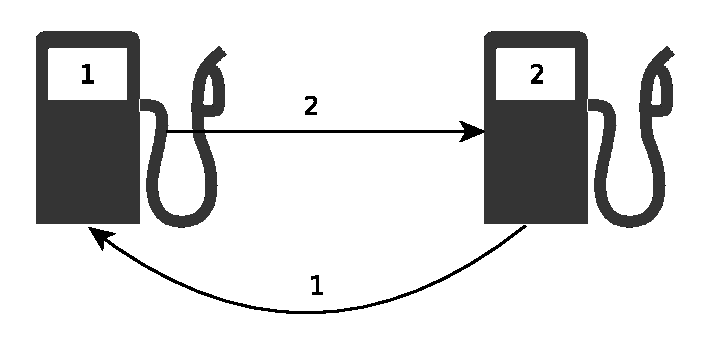
\includegraphics[width=\textwidth]{sources/gas_station/images/example1}
	\caption[Implicit graph for the Example \ref{example:gas_station:example1}.]
	{Visual representation the problem instance of Example
	\ref{example:gas_station:example1}.}.
	\label{fig:gas_station:example1}
\end{figure}

\begin{figure}
	\centering
	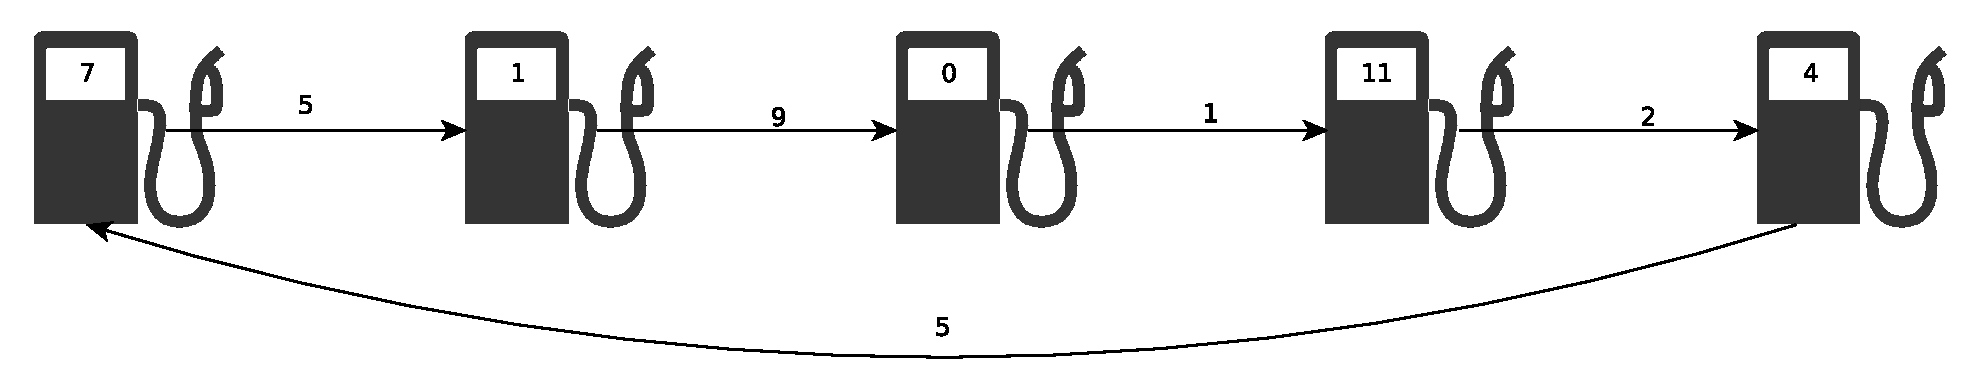
\includegraphics[width=\textwidth]{sources/gas_station/images/example2}
	\caption[Implicit graph for the Example \ref{example:gas_station:example2}.]
	{Visual representation the problem instance of Example
	\ref{example:gas_station:example2}.}.
	\label{fig:gas_station:example2}
\end{figure}

\section{Clarification Questions}

\begin{QandA}
	\item What shall the function return when it is not possible to complete a loop starting from any station? 
	\begin{answered}
		\textit{The function returns $-1$ in this case.}
	\end{answered}

	\item What is the maximum possible number of gas stations?
	\begin{answered}
		\textit{$n$ can be up to $1000000$.}
	\end{answered}

	\item Can we have negative values for gas refuel and cost?
	\begin{answered}
		\textit{No, you can assume $G$ and $C$ always contain non-negative integers.}
	\end{answered}
	
	\item Can $G$ and $C$ be empty?
	\begin{answered}
		\textit{Yes, $n$ can be zero.}
	\end{answered}
\end{QandA}

\section*{Discussion}
\label{gas_station:sec:discussion}
We can start our discussion by noticing that there are certain cases where it is impossible to perform a full loop, and specifically this is the case when the overall costs are higher than the total sum of available gas along the route. 
Clearly this signal the fact that we need more gas than it is available to complete the route. In this case we can return $-1$.

But are we guaranteed to be able to complete a loop if the available gas is more than the overall cost? The answer is a sound yes.

Moreover when there is only a single station in the route, we can immediately return $0$,regardless of the value we have in $C$, as in order to complete the loop we do not need to move our car at all.

\subsection{Brute-force}
\label{gas_station:sec:bruteforce}
A brute-force solution just simulates the car driving. We can perform this simulation by trying each time a different starting gas station. 

The simulation takes care of keeping track of the amount of gas in the tank as we move from station to station and it is implemented in function \inline{can_complete_loop_from_station} in Listing \ref{list:gas_station}.
This function is called from within a loop feeding it each time with a new starting gas station until either we tried them all or we found one from which is possible to complete a loop. The full implementation is shown in Listing \ref{list:gas_station}.


\lstinputlisting[language=c++, caption={Brute-force solution.},label=list:gas_station]{sources/gas_station/gas_station_solution1.cpp}

This solution has a time complexity of $O(n^2)$. The space complexity is constant.


\subsection{Linear time}
\label{gas_station:sec:linear_time}
Let's have a look at the brute-solution and see if we can find any ineficiencies and fix them. 
At a closer look it appears that, if we simulatates the car driving starting from a startion $k$ and we are able to drive it up until station $k+x$ then we stop and we start over simulation choosing as a starting point the station at index $k+1$. 
Is it really necessary? What if we could somehow start from $k+x$ and still be guaranteed we are not missing any potential good starting gas station?

Let's imagine for a second that we start from station $0$ are we are able to drive it up until station $3$ but we run out of gas when trying to drive to station $4$ as shown in Figure \ref{fig:gas_station:example_expl1}. When the brute-force simulation figures that is impossible to continue, it starts the simulation process from the second station (marked as B). But this simulation is useless and it is destined to also fail. Why is that? The reason is that we already know that with the first three legs of the trip we are already in a surplus or at the very least breaking even with the fuel amount. This is because if we were at some kind of deficit we would have not been able to make the three legs journey in the first place.

\begin{figure}
	\centering
	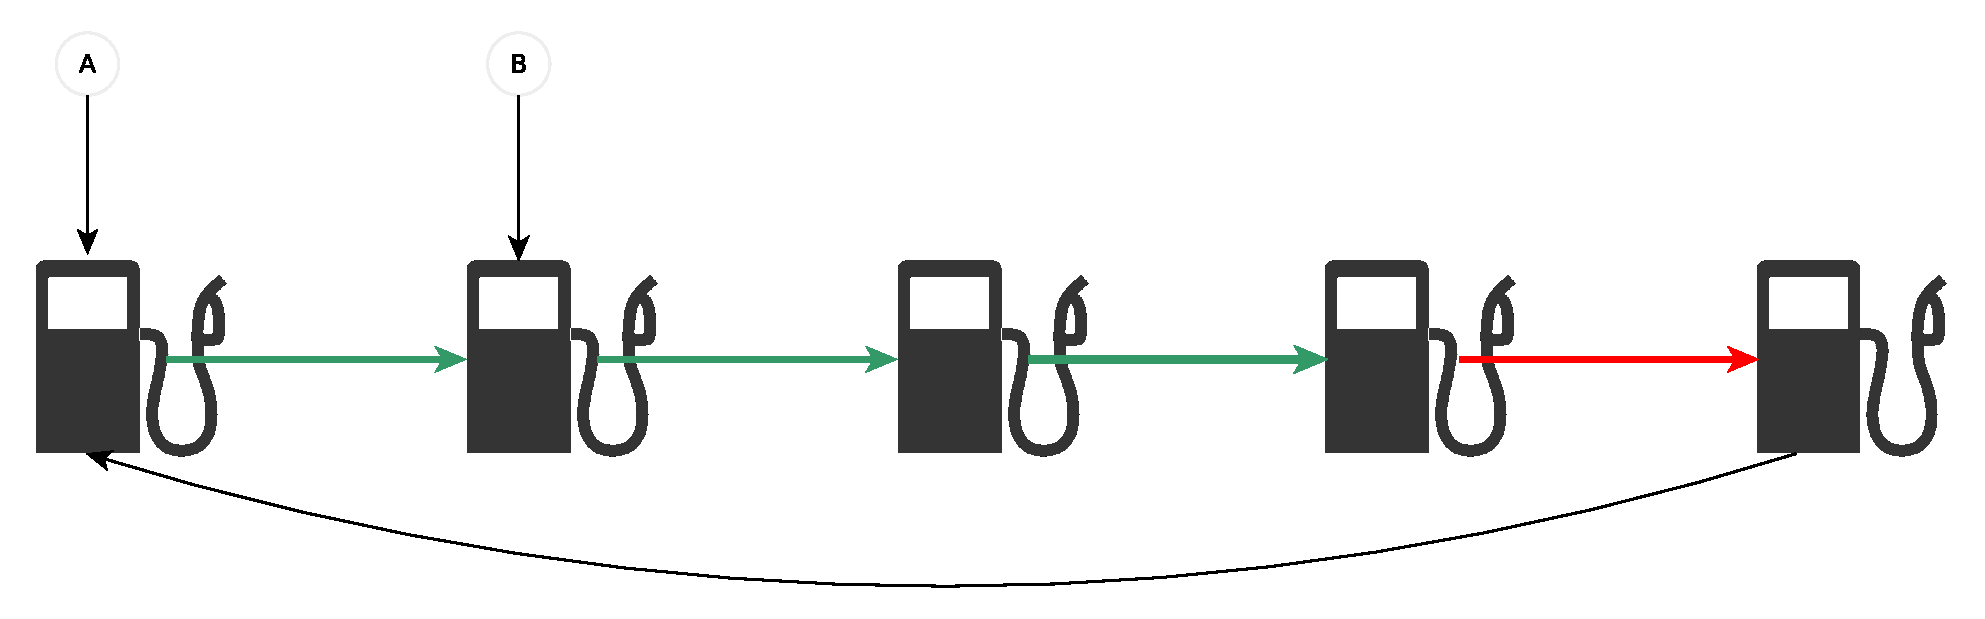
\includegraphics[width=\textwidth]{sources/gas_station/images/example_expl1}
	\caption[]{Behavior of the brute-force solution.}.
	\label{fig:gas_station:fig:gas_station:example_expl1}
\end{figure}

Therefore starting from station $1$ is not useful as in the previous simulation we arrived at station $1$ (starting from station $0$) with an amount of fuel greater or equal than zero. The same reasoning can be applied to the starting point $2$. Because when we simulated the car driving starting from station $0$ we were able to reach station $3$, this means we reached station $2$ from station $1$ with a surplus of fuel and therefore if we did not make it back then to station $4$, there is no way we can make it now that we start with $0$ liters of fuel from station $2$.

What does this mean in term of our algorithm? We know that when performing the simulation from station $k$, if we run out of fuel at station $k+x$ we can safely start our simulation at index $k+x+1$, saving a lot of work in the process. 
Moreover, when we finally are able to reach station $0$ again, we can immediately return the last starting station. 
For instance let's analyze the example shown in Figure \ref{fig:gas_station:fig:gas_station:example_expl2}. When starting from station $0$ we are able to make it up to station $3$. We then use station $4$ as starting point and we make it back to station $0$. We can at this point conclude that station $4$ is the answer because we know that there is an answer for this instance (the sum of the gas is greater or equal than the sum of the costs) and all the previous stations are not valid starting points. 

One can however argue that station $4$ (marked with a green circle) is not a valid starting point because we did not actually check we can make the journey from station $0$ to station $4$ (stations highlighted in light yellow) once we circled back and that maybe station $5$ (in cyan) or $6$ (in blue) are the right station to start from.
This reasoning is not quite right as again, if we make it to station $5$ or $6$ starting from station $4$, it means we reach those station with some sort of fuel surplus and therefore starting from station $5$ or $6$ would not be more beneficial than starting from station $4$.

All these insights above are implemented into a solution in Listing \ref{list:gas_station}.

\begin{figure}
	\centering
	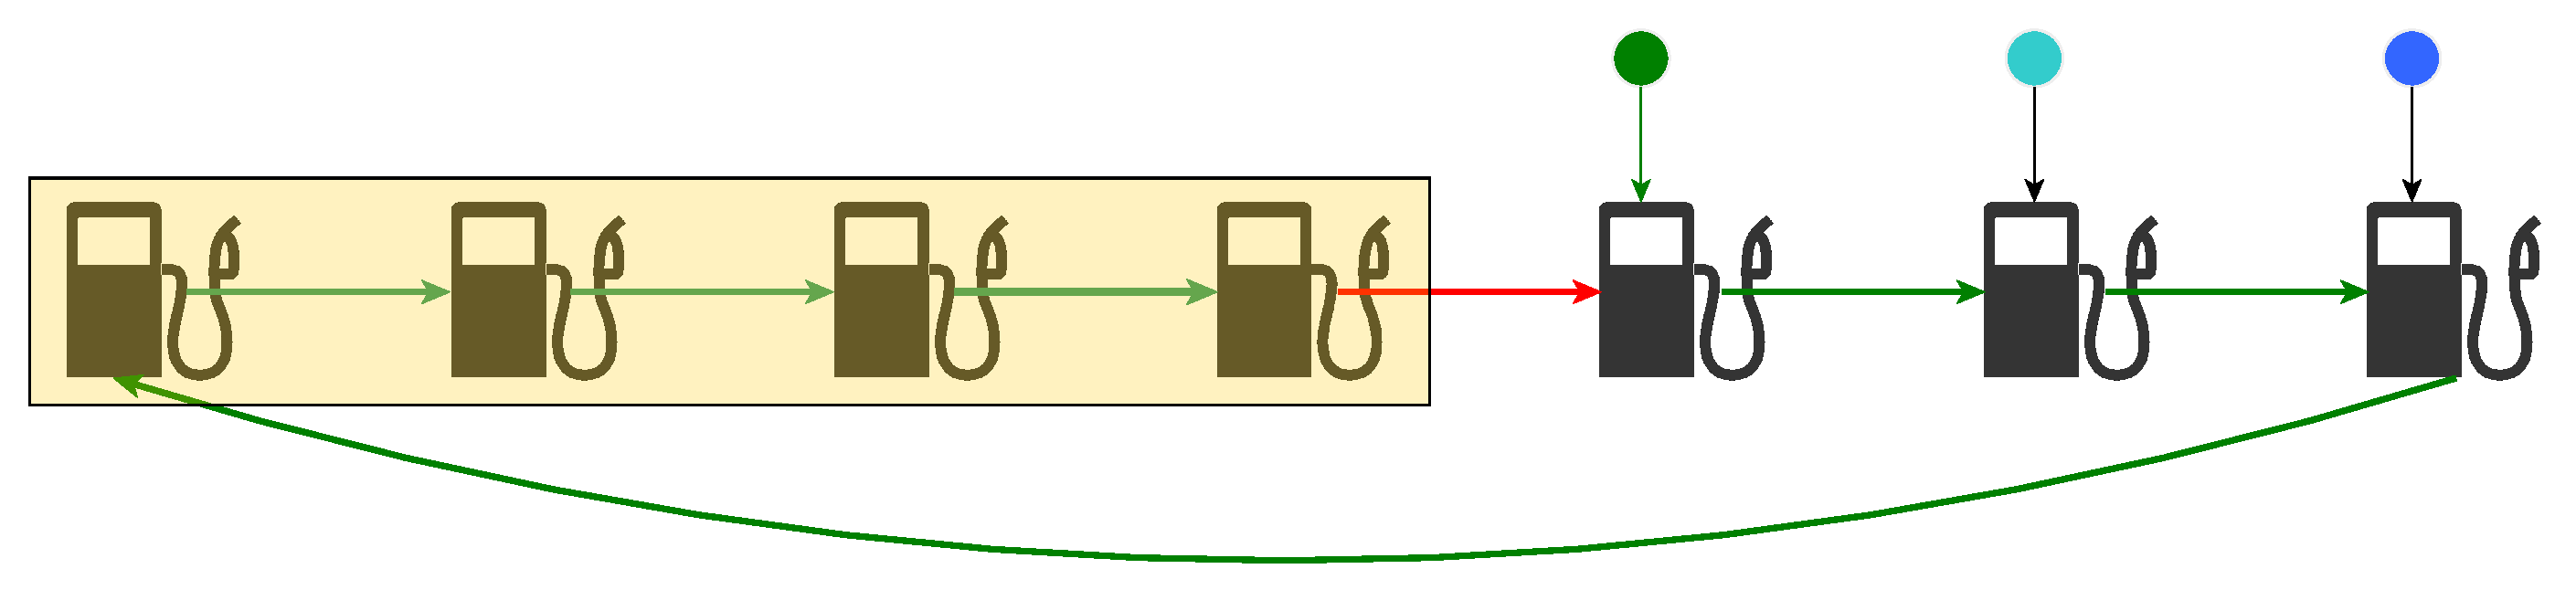
\includegraphics[width=\textwidth]{sources/gas_station/images/example_expl2}
	\caption[]{Behavior of the brute-force solution.}.
	\label{fig:gas_station:fig:gas_station:example_expl2}
\end{figure}



\lstinputlisting[language=c++, caption={Linear time constant space solution.},label=list:gas_station:linear]{sources/gas_station/gas_station_solution2.cpp}


\section{Common Variation - Fuel tank with limited capacity}

\begin{exercise}
	\label{example:gas_station:exercice1}
	Solve the problem described in Exercise \ref{} with the additional constraint that the fuel tank of the car has a maximum capacity $k$ that is given as an additional parameter to the function you need to write. 
\end{exercise}